\documentclass[12pt, a4paper]{report}
\usepackage{hyperref}
\usepackage[top=3cm,right=3cm,bottom=3cm,left=2.5cm]{geometry}
\usepackage{caption}
\usepackage{indentfirst}
\usepackage{graphicx}
\usepackage{subfigure}
\usepackage{float}
\usepackage{fancyhdr}
\usepackage{titlesec}
\usepackage{tikz}
\setcounter{secnumdepth}{4}
\setcounter{tocdepth}{4}


\pagestyle{fancy}
% Set up fancyhdr to place page number at the top left
\pagestyle{fancy}
\fancyhf{} % Clear all header/footer fields
\fancyhead[L]{\thepage} % Page number on the top left

% Define custom style for chapter page (no header or footer)
\fancypagestyle{plain}{
	\fancyhf{} % Clear headers and footers
	\renewcommand{\headrulewidth}{0pt} % Remove header rule
}


% Changing TOC addressing format (from period separation to dash seperation)
\renewcommand{\thesection}{\thechapter-\arabic{section}-}
\renewcommand{\thesubsection}{\thechapter-\arabic{section}-\arabic{subsection}-}
\renewcommand{\thesubsubsection}{\thechapter-\arabic{section}-\arabic{subsection}-\arabic{subsubsection}-}

\renewcommand{\thetable}{(\thechapter-\arabic{table})}

% Redefine how captions are written 
\renewcommand{\thefigure}{(\thechapter-\arabic{figure})}

% Set caption font size to 11pt
\captionsetup{font=small, labelsep=space} % 'small' is equivalent to 11pt in most classes

% Automatically switch between Persian and Latin fonts based on character type
\XeTeXinterchartokenstate=1
\newXeTeXintercharclass\persianchars
\newXeTeXintercharclass\latinchars

% Automatically switch fonts when switching between Persian and Latin characters
\XeTeXinterchartoks \latinchars \persianchars = {\begingroup\persianfont\endgroup}
\XeTeXinterchartoks \persianchars \latinchars = {\begingroup\latinfont\endgroup}



\title{Trust Compiler Report}
\author{InFluX}

\begin{document}
%\maketitle
\begin{titlepage}
	\centering
	% University logo
	\includegraphics[width=0.15\textwidth]{images/logo.png}
	
	% University and Faculty name
	{\Large Isfahan University}\par
	{\Large Computer Engineering Department}\par\vspace{2cm}
	
	% Report title
	\textbf
	{\Huge Trust Compiler Report}\par\vspace{1.5cm}
	
	% Intern details
	\large
	\textbf{Students:}\par{Zahra Masoumi - Matin Azami}\par\vspace{0.5cm}  
	\textbf{Students ID:}\par{4003623003 - 4003623003}\par\vspace{0.5cm}
	\textbf{Professor:}\par{Dr. Shafiee}\par\vspace{0.5cm}
		
	\par\vspace{2cm}
	
	
\end{titlepage}

\tableofcontents

\listoftables

\listoffigures


\chapter{Lexical Analyzer}

\section{Introduction}

\section{White Spaces}


\begin{center}
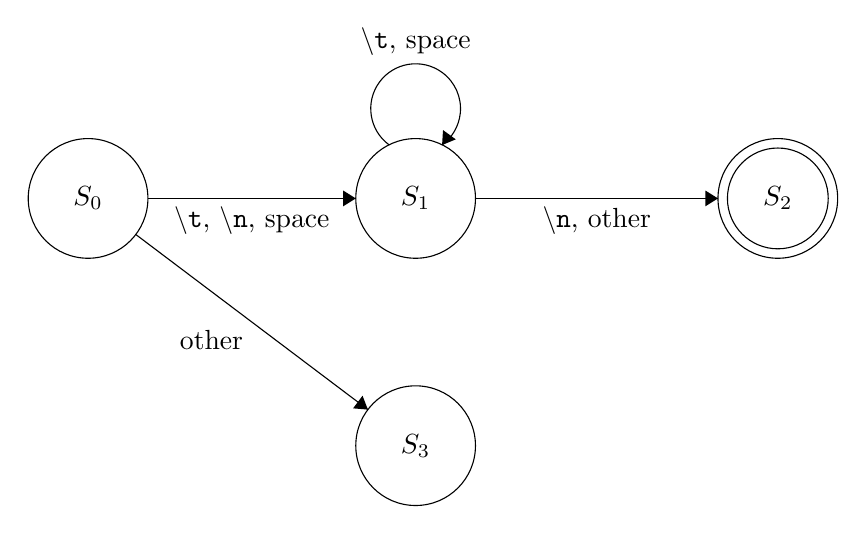
\begin{tikzpicture}[scale=0.2]
\tikzstyle{every node}+=[inner sep=0pt]
\draw [black] (4,-10.9) circle (3.8);
\draw (4,-10.9) node {$S_0$};
\draw [black] (24.8,-10.9) circle (3.8);
\draw (24.8,-10.9) node {$S_1$};
\draw [black] (47.8,-10.9) circle (3.8);
\draw (47.8,-10.9) node {$S_2$};
\draw [black] (47.8,-10.9) circle (3.2);
\draw [black] (24.8,-26.6) circle (3.8);
\draw (24.8,-26.6) node {$S_3$};
\draw [black] (7.8,-10.9) -- (21,-10.9);
\fill [black] (21,-10.9) -- (20.2,-10.4) -- (20.2,-11.4);
\draw (14.4,-11.4) node [below] {\texttt{\textbackslash t},\ \texttt{\textbackslash n},\ space};
\draw [black] (28.6,-10.9) -- (44,-10.9);
\fill [black] (44,-10.9) -- (43.2,-10.4) -- (43.2,-11.4);
\draw (36.3,-11.4) node [below] {\texttt{\textbackslash n},\ other};
\draw [black] (23.125,-7.506) arc (234:-54:2.85);
\draw (24.8,-1.85) node [above] {\texttt{\textbackslash t},\ space};
\fill [black] (26.48,-7.51) -- (27.35,-7.15) -- (26.54,-6.56);
\draw [black] (7.03,-13.19) -- (21.77,-24.31);
\fill [black] (21.77,-24.31) -- (21.43,-23.43) -- (20.83,-24.23);
\draw (11.84,-19.25) node [below] {other};
\end{tikzpicture}
\end{center}


\section{Comments}

\begin{center}
\begin{tikzpicture}[scale=0.2]
\tikzstyle{every node}+=[inner sep=0pt]
\draw [black] (4,-10.9) circle (3.8);
\draw (4,-10.9) node {$S_0$};
\draw [black] (19.9,-10.9) circle (3.8);
\draw (19.9,-10.9) node {$S_1$};
\draw [black] (35.8,-10.9) circle (3.8);
\draw (35.8,-10.9) node {$S_2$};
\draw [black] (51.2,-10.9) circle (3.8);
\draw (51.2,-10.9) node {$S_3$};
\draw [black] (19.9,-26.3) circle (3.8);
\draw (19.9,-26.3) node {$S_4$};
\draw [black] (7.8,-10.9) -- (16.1,-10.9);
\fill [black] (16.1,-10.9) -- (15.3,-10.4) -- (15.3,-11.4);
\draw (11.95,-11.4) node [below] {$/$};
\draw [black] (23.7,-10.9) -- (32,-10.9);
\fill [black] (32,-10.9) -- (31.2,-10.4) -- (31.2,-11.4);
\draw (27.85,-11.4) node [below] {$/$};
\draw [black] (39.6,-10.9) -- (47.4,-10.9);
\fill [black] (47.4,-10.9) -- (46.6,-10.4) -- (46.6,-11.4);
\draw (43.5,-11.4) node [below] {\texttt{\textbackslash n}};
\draw [black] (6.73,-13.54) -- (17.17,-23.66);
\fill [black] (17.17,-23.66) -- (16.94,-22.74) -- (16.25,-23.46);
\draw (9.38,-19.08) node [below] {$other$};
\draw [black] (19.9,-14.7) -- (19.9,-22.5);
\fill [black] (19.9,-22.5) -- (20.4,-21.7) -- (19.4,-21.7);
\draw (19.4,-18.6) node [left] {$other$};
\draw [black] (34.125,-7.506) arc (234:-54:2.85);
\draw (35.8,-1.85) node [above] {$other,\mbox{ }/$};
\fill [black] (37.48,-7.51) -- (38.35,-7.15) -- (37.54,-6.56);
\end{tikzpicture}
\end{center}


\section{Operators}

\subsection{Arithmetic Operations}

\subsection{Punctuation Marks}

\section{Numeric Values}

\subsection{HexaDecimal}

\subsection{Decimal}

\section{Keywords}

\begin{center}
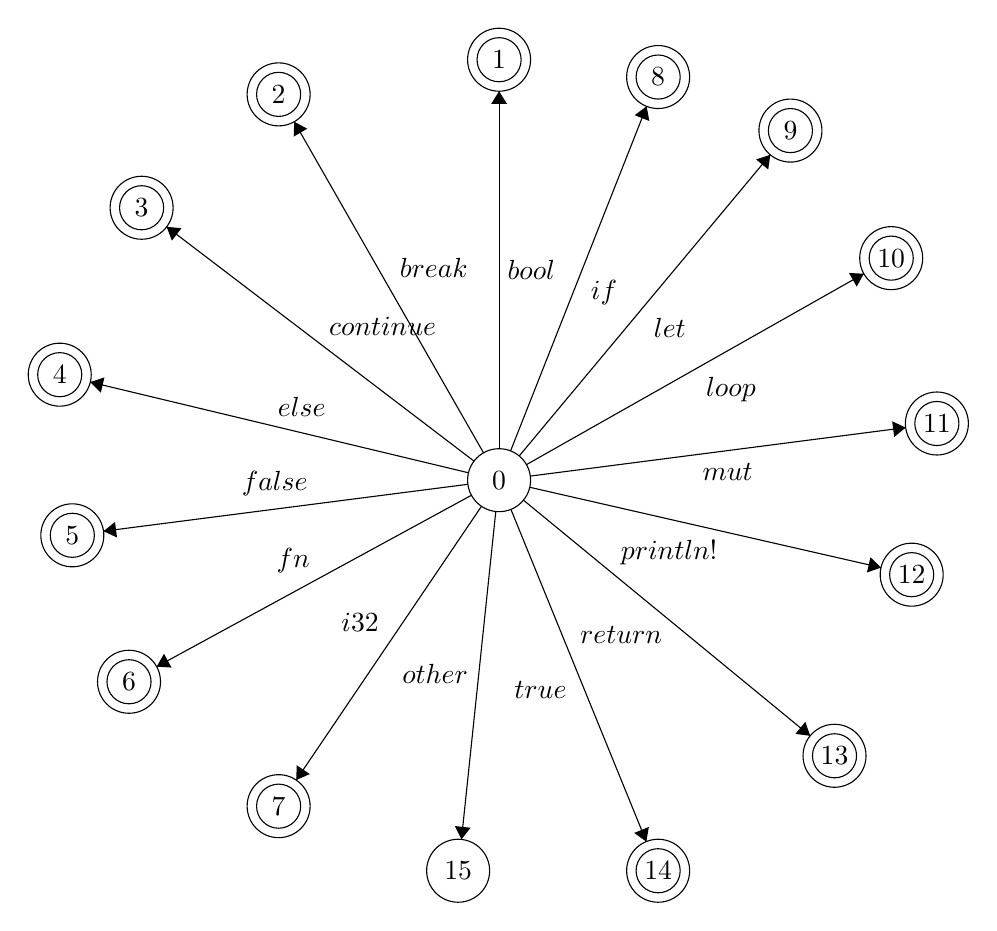
\begin{tikzpicture}[scale=0.2]
\tikzstyle{every node}+=[inner sep=0pt]
\draw [black] (30.1,-28.7) circle (2);
\draw (30.1,-28.7) node {$0$};
\draw [black] (30.1,-2) circle (2);
\draw (30.1,-2) node {$1$};
\draw [black] (30.1,-2) circle (1.4);
\draw [black] (16.1,-4.2) circle (2);
\draw (16.1,-4.2) node {$2$};
\draw [black] (16.1,-4.2) circle (1.4);
\draw [black] (7.4,-11.4) circle (2);
\draw (7.4,-11.4) node {$3$};
\draw [black] (7.4,-11.4) circle (1.4);
\draw [black] (2.2,-22) circle (2);
\draw (2.2,-22) node {$4$};
\draw [black] (2.2,-22) circle (1.4);
\draw [black] (3,-32.2) circle (2);
\draw (3,-32.2) node {$5$};
\draw [black] (3,-32.2) circle (1.4);
\draw [black] (6.6,-41.5) circle (2);
\draw (6.6,-41.5) node {$6$};
\draw [black] (6.6,-41.5) circle (1.4);
\draw [black] (16.1,-49.4) circle (2);
\draw (16.1,-49.4) node {$7$};
\draw [black] (16.1,-49.4) circle (1.4);
\draw [black] (27.5,-53.5) circle (2);
\draw (27.5,-53.5) node {$15$};
\draw [black] (40.2,-3.1) circle (2);
\draw (40.2,-3.1) node {$8$};
\draw [black] (40.2,-3.1) circle (1.4);
\draw [black] (48.6,-6.5) circle (2);
\draw (48.6,-6.5) node {$9$};
\draw [black] (48.6,-6.5) circle (1.4);
\draw [black] (55,-14.6) circle (2);
\draw (55,-14.6) node {$10$};
\draw [black] (55,-14.6) circle (1.4);
\draw [black] (57.9,-25.1) circle (2);
\draw (57.9,-25.1) node {$11$};
\draw [black] (57.9,-25.1) circle (1.4);
\draw [black] (56.3,-34.7) circle (2);
\draw (56.3,-34.7) node {$12$};
\draw [black] (56.3,-34.7) circle (1.4);
\draw [black] (51.4,-46.2) circle (2);
\draw (51.4,-46.2) node {$13$};
\draw [black] (51.4,-46.2) circle (1.4);
\draw [black] (40.2,-53.5) circle (2);
\draw (40.2,-53.5) node {$14$};
\draw [black] (40.2,-53.5) circle (1.4);
\draw [black] (30.1,-26.7) -- (30.1,-4);
\fill [black] (30.1,-4) -- (29.6,-4.8) -- (30.6,-4.8);
\draw (30.6,-15.35) node [right] {$bool$};
\draw [black] (29.11,-26.96) -- (17.09,-5.94);
\fill [black] (17.09,-5.94) -- (17.06,-6.88) -- (17.92,-6.38);
\draw (23.76,-15.23) node [right] {$break$};
\draw [black] (28.51,-27.49) -- (8.99,-12.61);
\fill [black] (8.99,-12.61) -- (9.32,-13.49) -- (9.93,-12.7);
\draw (22.7,-19.55) node [above] {$continue$};
\draw [black] (28.16,-28.23) -- (4.14,-22.47);
\fill [black] (4.14,-22.47) -- (4.81,-23.14) -- (5.04,-22.17);
\draw (17.57,-24.7) node [above] {$else$};
\draw [black] (28.12,-28.96) -- (4.98,-31.94);
\fill [black] (4.98,-31.94) -- (5.84,-32.34) -- (5.71,-31.35);
\draw (15.85,-29.73) node [above] {$false$};
\draw [black] (28.34,-29.66) -- (8.36,-40.54);
\fill [black] (8.36,-40.54) -- (9.3,-40.6) -- (8.82,-39.72);
\draw (17.02,-34.6) node [above] {$fn$};
\draw [black] (28.98,-30.36) -- (17.22,-47.74);
\fill [black] (17.22,-47.74) -- (18.08,-47.36) -- (17.25,-46.8);
\draw (22.49,-37.71) node [left] {$i32$};
\draw [black] (30.83,-26.84) -- (39.47,-4.96);
\fill [black] (39.47,-4.96) -- (38.71,-5.52) -- (39.64,-5.89);
\draw (35.9,-16.77) node [right] {$if$};
\draw [black] (31.38,-27.16) -- (47.32,-8.04);
\fill [black] (47.32,-8.04) -- (46.42,-8.33) -- (47.19,-8.97);
\draw (39.9,-19.04) node [right] {$let$};
\draw [black] (31.84,-27.71) -- (53.26,-15.59);
\fill [black] (53.26,-15.59) -- (52.32,-15.54) -- (52.81,-16.41);
\draw (44.82,-22.15) node [below] {$loop$};
\draw [black] (32.08,-28.44) -- (55.92,-25.36);
\fill [black] (55.92,-25.36) -- (55.06,-24.96) -- (55.19,-25.96);
\draw (44.61,-27.59) node [below] {$mut$};
\draw [black] (32.05,-29.15) -- (54.35,-34.25);
\fill [black] (54.35,-34.25) -- (53.68,-33.59) -- (53.46,-34.56);
\draw (40.9,-32.47) node [below] {$println!$};
\draw [black] (31.65,-29.97) -- (49.85,-44.93);
\fill [black] (49.85,-44.93) -- (49.55,-44.04) -- (48.92,-44.81);
\draw (37.85,-37.94) node [below] {$return$};
\draw [black] (30.85,-30.55) -- (39.45,-51.65);
\fill [black] (39.45,-51.65) -- (39.61,-50.72) -- (38.68,-51.1);
\draw (34.41,-42) node [left] {$true$};
\draw [black] (29.89,-30.69) -- (27.71,-51.51);
\fill [black] (27.71,-51.51) -- (28.29,-50.77) -- (27.29,-50.66);
\draw (28.15,-41) node [left] {$other$};
\end{tikzpicture}
\end{center}

\section{Strings}

\begin{center}
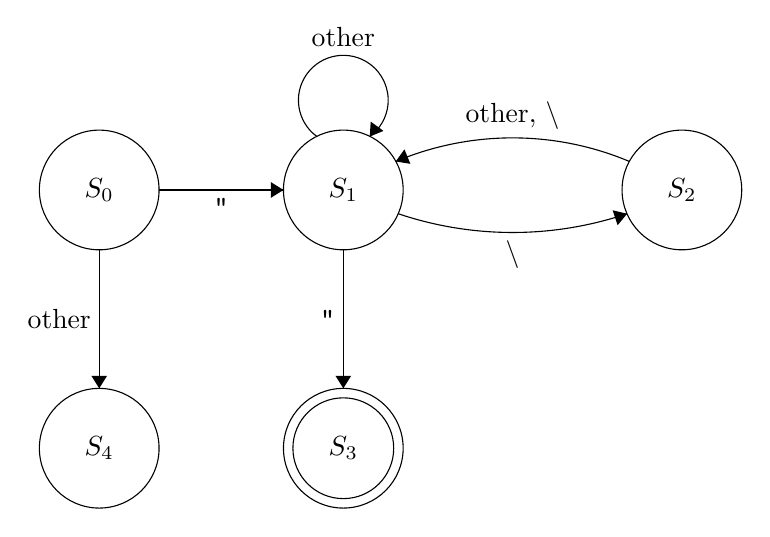
\begin{tikzpicture}[scale=0.2]
\tikzstyle{every node}+=[inner sep=0pt]
\draw [black] (4.7,-10.9) circle (3.8);
\draw (4.7,-10.9) node {$S_0$};
\draw [black] (20.2,-10.9) circle (3.8);
\draw (20.2,-10.9) node {$S_1$};
\draw [black] (41.7,-10.9) circle (3.8);
\draw (41.7,-10.9) node {$S_2$};
\draw [black] (20.2,-27.3) circle (3.8);
\draw (20.2,-27.3) node {$S_3$};
\draw [black] (20.2,-27.3) circle (3.2);
\draw [black] (4.7,-27.3) circle (3.8);
\draw (4.7,-27.3) node {$S_4$};
\draw [black] (8.5,-10.9) -- (16.4,-10.9);
\fill [black] (16.4,-10.9) -- (15.6,-10.4) -- (15.6,-11.4);
\draw (12.45,-11.4) node [below] {\texttt{"}};
\draw [black] (4.7,-14.7) -- (4.7,-23.5);
\fill [black] (4.7,-23.5) -- (5.2,-22.7) -- (4.2,-22.7);
\draw (4.2,-19.1) node [left] {other};
\draw [black] (18.525,-7.506) arc (234:-54:2.85);
\draw (20.2,-1.85) node [above] {other};
\fill [black] (21.88,-7.51) -- (22.75,-7.15) -- (21.94,-6.56);
\draw [black] (38.217,-12.408) arc (-71.36814:-108.63186:22.746);
\fill [black] (38.22,-12.41) -- (37.3,-12.19) -- (37.62,-13.14);
\draw (30.95,-14.1) node [below] {\texttt{\textbackslash}};
\draw [black] (20.2,-14.7) -- (20.2,-23.5);
\fill [black] (20.2,-23.5) -- (20.7,-22.7) -- (19.7,-22.7);
\draw (19.7,-19.1) node [left] {\texttt{"}};
\draw [black] (23.533,-9.089) arc (112.82624:67.17376:19.118);
\fill [black] (23.53,-9.09) -- (24.46,-9.24) -- (24.08,-8.32);
\draw (30.95,-7.09) node [above] {other, \texttt{\textbackslash}};
\end{tikzpicture}
\end{center}


\section{IDs}


\end{document}